\documentclass[12pt]{article}\usepackage[]{graphicx}\usepackage[]{color}
%% maxwidth is the original width if it is less than linewidth
%% otherwise use linewidth (to make sure the graphics do not exceed the margin)
\makeatletter
\def\maxwidth{ %
  \ifdim\Gin@nat@width>\linewidth
    \linewidth
  \else
    \Gin@nat@width
  \fi
}
\makeatother

\definecolor{fgcolor}{rgb}{0.345, 0.345, 0.345}
\newcommand{\hlnum}[1]{\textcolor[rgb]{0.686,0.059,0.569}{#1}}%
\newcommand{\hlstr}[1]{\textcolor[rgb]{0.192,0.494,0.8}{#1}}%
\newcommand{\hlcom}[1]{\textcolor[rgb]{0.678,0.584,0.686}{\textit{#1}}}%
\newcommand{\hlopt}[1]{\textcolor[rgb]{0,0,0}{#1}}%
\newcommand{\hlstd}[1]{\textcolor[rgb]{0.345,0.345,0.345}{#1}}%
\newcommand{\hlkwa}[1]{\textcolor[rgb]{0.161,0.373,0.58}{\textbf{#1}}}%
\newcommand{\hlkwb}[1]{\textcolor[rgb]{0.69,0.353,0.396}{#1}}%
\newcommand{\hlkwc}[1]{\textcolor[rgb]{0.333,0.667,0.333}{#1}}%
\newcommand{\hlkwd}[1]{\textcolor[rgb]{0.737,0.353,0.396}{\textbf{#1}}}%

\usepackage{framed}
\makeatletter
\newenvironment{kframe}{%
 \def\at@end@of@kframe{}%
 \ifinner\ifhmode%
  \def\at@end@of@kframe{\end{minipage}}%
  \begin{minipage}{\columnwidth}%
 \fi\fi%
 \def\FrameCommand##1{\hskip\@totalleftmargin \hskip-\fboxsep
 \colorbox{shadecolor}{##1}\hskip-\fboxsep
     % There is no \\@totalrightmargin, so:
     \hskip-\linewidth \hskip-\@totalleftmargin \hskip\columnwidth}%
 \MakeFramed {\advance\hsize-\width
   \@totalleftmargin\z@ \linewidth\hsize
   \@setminipage}}%
 {\par\unskip\endMakeFramed%
 \at@end@of@kframe}
\makeatother

\definecolor{shadecolor}{rgb}{.97, .97, .97}
\definecolor{messagecolor}{rgb}{0, 0, 0}
\definecolor{warningcolor}{rgb}{1, 0, 1}
\definecolor{errorcolor}{rgb}{1, 0, 0}
\newenvironment{knitrout}{}{} % an empty environment to be redefined in TeX

\usepackage{alltt}  
\usepackage{amsfonts, amsmath, amsthm, amssymb, enumitem, verbatim, graphicx}
\setlength{\parindent}{0pt}
\setlength{\parskip}{1ex plus 0.5ex minus 0.2ex}
\usepackage [margin=1in, paperwidth=8.5in, paperheight=11in]{geometry}

\newcommand{\bfbeta}{\mbox{\boldmath $\beta$}}
\newcommand{\bfX}{\mbox{\boldmath $X$}}
\newcommand{\bfx}{\mbox{\boldmath $x$}}
\newcommand{\bfV}{\mbox{\boldmath $V$}}
\newcommand{\bfI}{\mbox{\boldmath $I$}}
\newcommand{\bfy}{\mbox{\boldmath $y$}}
\newcommand{\bfeps}{\mbox{\boldmath $\epsilon$}}
\IfFileExists{upquote.sty}{\usepackage{upquote}}{}
\begin{document}


{ \flushright Jordan Schupbach \\
STAT 532\\
September 21, 2015 \\}
Homework \# 3\\

\begin{enumerate}
\item The authors of the paper I chose use two sets of priors. In both, they are simply using the prior as an adjustment to the mean performance of market benchmarks for 3 crops: corn, wheat and soybean. The authors write that "there are two levels of parameters in the normal hierarchical model for market advidory service performance. The expected performance of each advisory program $\theta = (\theta_1, \dots, \theta_n)$, in the lower level, ... and hyperparameters $(\mu, \tau)$" in the normal model where
\[ \theta_j | \mu, \tau \sim N(\mu, \tau^2) \]
In the first set considered, a normal prior is used, with uninformed hyperparamters. For the mean of their prior, they use a uniform prior with no truncation. They argue this is reasonable as their sample size is large enough to rely only one the sample for estimation of this parameter. They also use a uniform prior on the variance estimate, which, they argue (citing Gelman (2006)) is supposed to perform well whent the number of groups is larger than 2 or 3. They seem to do a reasonable job at arguing their choices of priors here. They write "The prior is based on the notion that performance across programs is not independent, but instead, data on pricing performance of a particular program as well as the performance of the rest of the programs are helpful in estimating expected performance." \\

In the second set of priors, they survey farmers (to elicit expert opinion) with two questions:
\begin{enumerate}[label = (\alph*)]
\item What is the most likely difference between the price obtained by following the recommendations of advisory programsand the market benchmark price? 
\item What is the probability that an advisory program outperforms the market benchmark, on average, by more than 5\%?
\end{enumerate}

They then use the mean of the first question as the hyperparameter on a normal prior and use both the mean of the first and the answer to the second question to form the variance hyperparameter. They say that they use the normal distribtion as a prior for "skeptical beliefs" as they say it simplifies computation of the posterior distribution. My main issue with this is that they then make no discussion of a sensitivity analysis to justify that this decision wouldn't greatly impact the posterior. 

\item My main take-away from this section is that if there are any simplifications made in specifying a prior (i.e. going with "non-informative or reference prior densities"), then the researcher ought to at least justify their choice, check that the posterior is proper, and perform a sensitivity analysis on priors for any modeling assumptions made out of convenience.

\item 
\begin{enumerate}[label = (\alph*)]
\item I do agree with Gelman's stance on weakly informative priors. To me, specifying priors has the same costs, benefits, and subjectivity as model specification, to which it is often reasonable to simplify model assumptions for a myriad of different reasons. For instance, we often may think a-priori that a quadratic model may fit the data, only to find out that we don't gain much prediction capability by this choice. We then may choose to go with the simpler model to simplify inferences made, even though the quadratic model has better fit. This is similar to the choice of not incorporating all prior information into a prior distribution. Sometimes the costs simply outweigh the benefits of incorporating model complexities.\\

Further, I like his advice on not using prior information heavily when it is part of the analysis. I've seen a number of studies (especially in the realm of social sciences), where it seems that the inferences made match too well to their prior beliefs. I often suspect in these cases that they are simply using data which they already have a good idea of what it should look like, to then support their argument being made. To me, I feel in these circumstances that one should "lean against the hypothesis" with prior specifications.

\item I think that Kenny's comments were reasonable in that it may be possible that the researchers made some more informed decisions about the prior specification than was lead on. Perhaps, as suggested by Gelman, they may be trying to "lean against the hypothesis" or that some simplification was made as the costs of incorporating this information would outweigh the benefits. However, in absence of access to the reasearchers, I think it would be reasonable to try to fit the data given better than the authors have done. After looking into this further, I actually came up with a fairly similar decision as far as parameters on the beta distribution. I think that the scaling on the y-axis of their graph just seems to be off, as I wouldn't see how either distribution (histogram or beta) sums to one. In looking at the distribution though, and making some rough estimates on quantiles, I came up with a beta(2.370455, 5.800109) distribution, which isn't all that dissimilar to what the authors of Kenny's paper came up with. Here's a plot of the author's choice versus mine. Code used is provided in the appendix.

\begin{knitrout}
\definecolor{shadecolor}{rgb}{0.969, 0.969, 0.969}\color{fgcolor}

{\centering 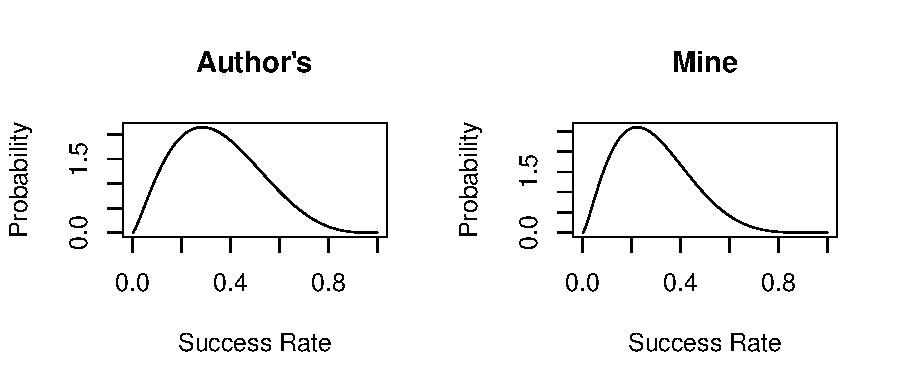
\includegraphics[width=\maxwidth]{figure/plot3-1} 

}



\end{knitrout}

I think that so long as there is enough data collected, these priors will work well enough. However, in the case of small sample sizes, we may need to take greater care and move away from the beta distribution.
\end{enumerate}
\item We use the following code to computationally approximate the parameters of the beta distribution which have the given characteristics. 

\begin{verbatim}
error_func <- function(v){
  abs(qbeta(.5,v[1],v[2]) - .3) + abs((1 - pbeta(.75, v[1], v[2])) - .1)
}

nlm(error_func, c(2,2), stepmax = 1, iterlim = 1000, gradtol = .000000001)

\end{verbatim}

We find that a $beta(0.7920481, 1.4748258)$ distribution reflects the two criterion given. A plot of this distribution is given below.

\begin{knitrout}
\definecolor{shadecolor}{rgb}{0.969, 0.969, 0.969}\color{fgcolor}

{\centering 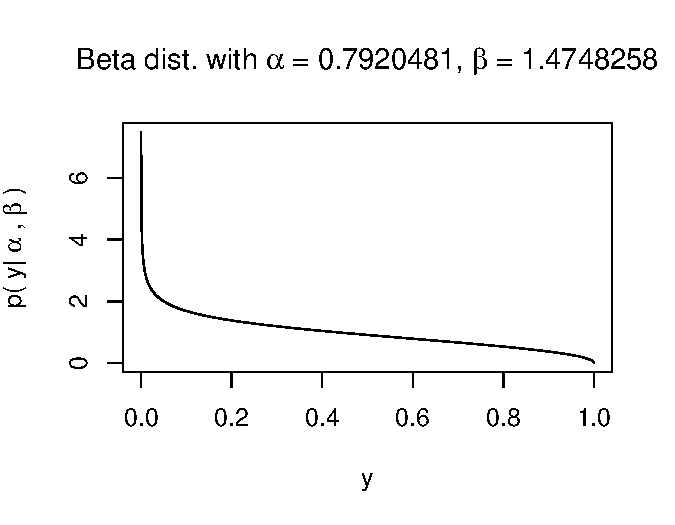
\includegraphics[width=\maxwidth]{figure/plot4-1} 

}



\end{knitrout}

\item
\begin{enumerate}[label = (\alph*)]
\item We have $y | \lambda \sim Pois(\lambda)$, which gives
\begin{align*}
P(y | \lambda) &= \dfrac{\lambda^y e^{- \lambda}}{y !}\\
& \propto \lambda^y e^{- \lambda}\\
&= e^{- \lambda} e^{y log \lambda}\\
&= g(\lambda)^n e^{\phi(\lambda)^T t(y)}
\end{align*}
and so, a prior density of the form
\begin{align*}
p(\lambda) &\propto g(\lambda)^{\beta} e^{\phi(\lambda)^T (\alpha - 1)}\\
&= (e^{-\lambda})^{\beta} e^{(log \lambda)(\alpha - 1)}\\
&= \underbrace{e^{- \lambda \beta} \lambda^{\alpha - 1}}_{\text{Kernel of } Gamma( \alpha, \beta)}
\end{align*}
is conjugate to the poisson pmf.

\item We have
\begin{align*}
p( \bfy | \lambda) &= \prod_{i = 1}^n \dfrac{ \lambda^{y_i} e^{- \lambda}}{y_i !}\\
&= \dfrac{\lambda^{\sum_{i=1}^n y_i} e^{- n \lambda}}{\prod_{i=1}^n y_i !}
\end{align*}
and so
\begin{align*}
p( \lambda | \bfy) &\propto \lambda^{\sum_{i=1}^n y_i} e^{-n \lambda} \lambda^{\alpha - 1} e^{- \lambda \beta}\\
&= \underbrace{\lambda^{\sum_{i=1}^n y_i + \alpha - 1} e^{-\lambda( n + \beta)}}_{\text{Kernel of } gamma( \sum_{i=1}^n y_i + \alpha, n + \beta)}
\end{align*}
Thus, we have $\lambda | \bfy \sim gamma( \sum_{i=1}^n y_i + \alpha, n + \beta)$

\item

\item I set the following criterion in the search for a gamma distribution: 
\begin{itemize}
\item The probability of $\lambda$ being between 15 and 25 as .80.
\item The probability of $\lambda$ being between 10 and 35 as .95.
\item The probability of $\lambda$ being between 15 and 25 as .99.
\end{itemize}

Then, I searched the parameter space to find a gamma distribution that closely matched those criterion. I obtained a $gamma(21.753974  ,1.075465)$ distribution.

\item I obtained the sample with the following R-code:

\begin{verbatim}
set.seed(2015)
samp1 <- rpois(20, rgamma(1, 21.753974  ,1.075465))
\end{verbatim}

\item Below, a histogram and a density plot are given for the data with a verticle line specifying the value of the sample drawn from the prior distribution.

\begin{knitrout}
\definecolor{shadecolor}{rgb}{0.969, 0.969, 0.969}\color{fgcolor}

{\centering 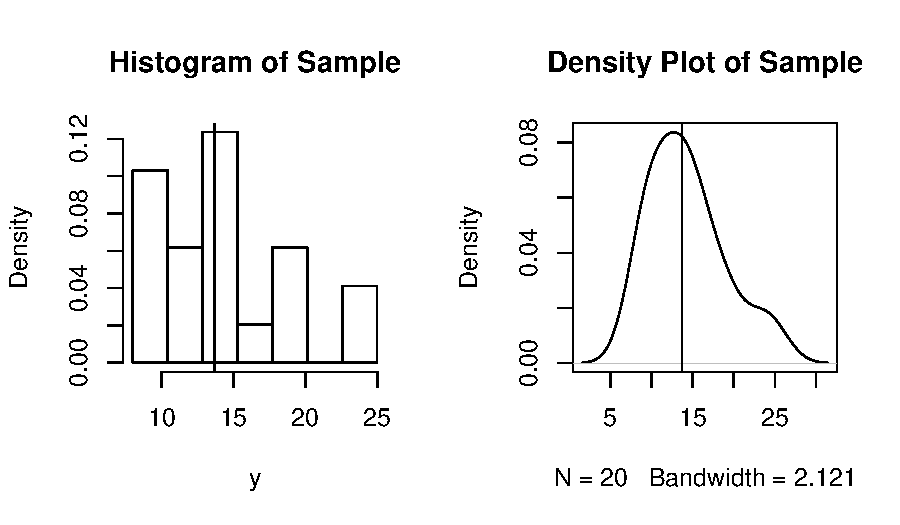
\includegraphics[width=\maxwidth]{figure/plot5f-1} 

}



\end{knitrout}

\item From our sample, we have that $\sum_{i=1}^{20} y_i= 286$ Thus, from the work in part (b), we know that 
\[ \lambda | \bfy \sim gamma(307.754, 21.075465) \]

We have the following plots of the likelihood, the posterior, and the prior.

\item

\item

\item


\item
\begin{enumerate}[label = \roman*.]
\item
\item
\end{enumerate}
\end{enumerate}

\item
\begin{enumerate}[label = (\alph*)]
\item
\item
\item
\item
\item
\item
\item
\end{enumerate}

\item
With the plot below, we illustrate the process of numerical integration. They are histograms of a very large sample drawn from the normal pdf with the associated pdf superimposed. Although these plots were made  with simply using the hist() and dnorm() functions in R, they are done in such a way to approximate what the graphs of a riemann sum would look like using the midpoint rule. We see that as our mesh grid is refined, our error associated with the process goes to zero. Thus, we can make our mesh grid so fine that our error is negligible. Note, that using the midpoint rule is superior to the left and right hand rules when the function we are numerically integrating is monotonic increasing or decreasing. There are also many other more efficient forms of numerical quadrature. 

\begin{knitrout}
\definecolor{shadecolor}{rgb}{0.969, 0.969, 0.969}\color{fgcolor}

{\centering 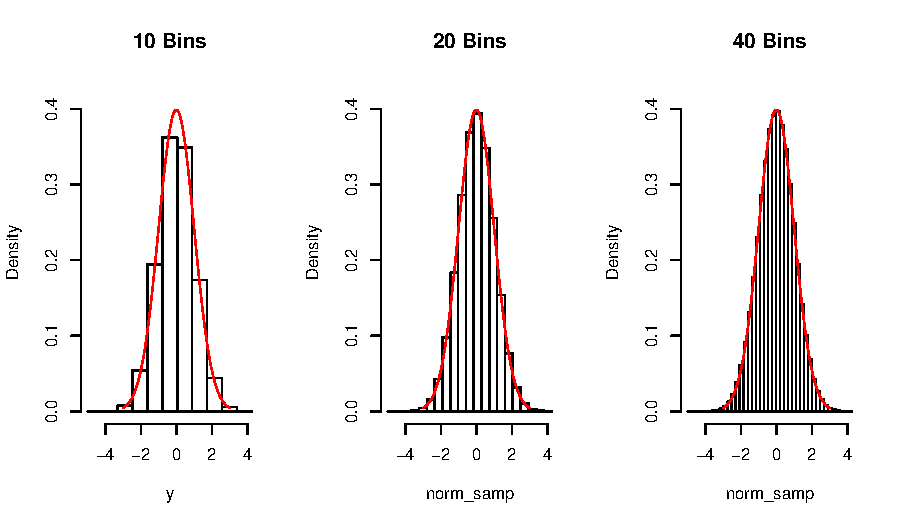
\includegraphics[width=\maxwidth]{figure/plot7-1} 

}



\end{knitrout}


\item 
\begin{enumerate}[label = (\alph*)]
\item
Yes, the resulting distribution would be proper. With $y| \theta \sim Bin(40, \theta)$, and $\theta \sim beta(0,0)$, we have
\begin{align*}
p(\theta | y) & \propto {n \choose y} \theta^y (1 - \theta)^{40 - y} \theta^{-1} (1 - \theta)^{-1}\\
& \propto \underbrace{\theta^{y - 1} (1 - \theta)^{40 - y - 1}}_{\text{Kernel of } beta(y, 40 - y)}
\end{align*}
Thus, if we observe $y = 10$, we have
\[ \theta | y \sim beta(10, 30) \]
Which is a proper distribution.
\item
No. If we observe $y =0$, we have $ \theta | y \sim beta(0, 40)$, which is not a proper distribution. We have
\begin{align*}
\int_0^1 (\theta)^{-1} (1 - \theta)^{39} (B(0, 40))^{-1} d \theta & = \int_0^1 (\theta)^{-1} (1 - \theta)^{39} d \theta\\
&= \int_0^1 \sum_{i = 0}^{38} \dfrac{{39 \choose i} ( - \theta)^{39 - i}}{\theta} d \theta + \int_0^1 \dfrac{1}{\theta} d \theta \\
&= \sum_{i = 0}^{38} \dfrac{ {39 \choose i} (-1)^{39 - i}}{39 - i} + \underset{b \rightarrow 0^+}{\text{lim}}  - ln(b)\\
&= - \dfrac{2066035355155033}{485721041551200} + \infty\\
&= \infty
\end{align*}
Thus, since the integral is not equal to one, $beta(0, 40)$ is not a proper distribution.
\item
Yes. We can simply use the following code:

\begin{verbatim}
f_x_8 <- function(x) ((1 - x)^39)/(x)
f_x_8_vec <- Vectorize(f_x_8)
integrate(f_x_8_vec, 10^(-15), 1)
\end{verbatim}
Which gives us that the integral is equal to "30.28523 with absolute error $< 0.0021$" for the given bounds.  Since this doesn't integrate to 1, we know that this is an improper prior. Note that I knew ahead of time that the problem was at zero and the second argument in the integrate() function, I used $10^{-15}$. If I hadn't known this ahead of time and put 0 in for this argument, I would have received the following error in R.

\begin{verbatim}
Error in integrate(f_x_8_vec, 0, 1) : 
  maximum number of subdivisions reached
\end{verbatim}

This error would also have told me that there may be a problem in the integral being equal to 1, as the function integrate() uses more subdivisions when the change in y is relatively large compared to the change in x.

\end{enumerate}
\item
\end{enumerate}
\newpage
\section*{R-Code}
\begin{verbatim}
R-Code Here
\end{verbatim}
\end{document})
